\documentclass[12pt,a4paper]{article}

% Packages
\usepackage[utf8]{inputenc}
\usepackage[T1]{fontenc}
\usepackage{amsmath,amssymb}
\usepackage{graphicx}
\usepackage{booktabs}
\usepackage{hyperref}
\usepackage{geometry}
\usepackage{natbib}
\usepackage{xcolor}
\usepackage{tikz}
\usepackage{pgfplots}
\usepackage{enumitem}
\usepackage{float}
\usepackage{caption}
\usepackage{subcaption}
\usepackage{longtable}
\usepackage{array}
\usepackage{multicol}
\usepackage{fancyhdr}
\usepackage{titlesec}

\pgfplotsset{compat=1.18}

\geometry{margin=1in}
\hypersetup{
    colorlinks=true,
    linkcolor=blue,
    filecolor=magenta,
    urlcolor=cyan,
    citecolor=blue
}

% Header and Footer
\pagestyle{fancy}
\fancyhf{}
\rhead{Email Cyber Attacks on Financial Institutions}
\lhead{Scientific Review}
\rfoot{Page \thepage}
\setlength{\headheight}{14.5pt}

% Title formatting
\titleformat{\section}{\large\bfseries}{\thesection}{1em}{}
\titleformat{\subsection}{\normalsize\bfseries}{\thesubsection}{1em}{}

\title{\textbf{Cybersecurity Threats via Email in Banks and Financial Institutions: \\A Comprehensive Scientific Review}}
\author{Deep Search Analysis\\
\small Sources: Google Scholar, ScienceDirect, arXiv, Dimensions, ResearchGate\\
\small Generated: January 2026}
\date{}

\begin{document}

\maketitle

\begin{abstract}
Financial institutions, particularly banks, represent prime targets for email-based cyber attacks due to their direct access to monetary assets and sensitive customer data. This comprehensive review examines the scientific literature on email cybersecurity threats specifically targeting the banking and financial sector. Drawing from peer-reviewed research in \textit{Computers \& Security}, \textit{Journal of Financial Crime}, \textit{Procedia Computer Science}, IEEE symposiums, and arXiv preprints, we analyze the evolution of phishing, Business Email Compromise (BEC), and malware attacks targeting financial institutions. The review covers attack taxonomies, financial impact assessments, machine learning detection approaches, employee awareness training effectiveness, and regulatory frameworks. Key findings indicate that financial institutions face annual losses exceeding \$2.7 billion from BEC attacks alone, with phishing remaining the primary initial attack vector in 91\% of successful breaches. We present evidence-based recommendations for comprehensive email security strategies in the banking sector.
\end{abstract}

\textbf{Keywords:} Cybersecurity, Email, Bank, Financial Institution, Phishing, Business Email Compromise, Fraud Detection, Machine Learning, Risk Management

\tableofcontents
\newpage

%==============================================================================
\section{Introduction}
%==============================================================================

The digital transformation of banking has created unprecedented opportunities for financial services delivery while simultaneously exposing institutions to sophisticated cyber threats. Email, as the primary communication channel for business operations, has become the most exploited attack vector targeting financial institutions \citep{gulyas2023impact}.

According to Gulyás and Kiss (2023), ``ransomware attacks that targeted banks and financial institutions'' have caused billions in losses globally, with email serving as the initial compromise vector in the majority of cases. The financial sector's unique position---handling monetary transactions and storing sensitive personal data---makes it particularly attractive to cybercriminals.

This review addresses the following research questions:
\begin{enumerate}[noitemsep]
    \item How have email-based cyber attacks targeting financial institutions evolved?
    \item What are the primary attack vectors and their financial impacts?
    \item What detection and prevention methodologies demonstrate effectiveness?
    \item How can financial institutions optimize their email security posture?
\end{enumerate}

%==============================================================================
\section{The Financial Sector Threat Landscape}
%==============================================================================

\subsection{Why Financial Institutions Are Targeted}

Financial institutions face disproportionate targeting for several reasons:

\begin{itemize}
    \item \textbf{Direct Monetary Access}: Banks can facilitate immediate fund transfers
    \item \textbf{High-Value Data}: Customer PII, account credentials, trading information
    \item \textbf{Regulatory Pressure}: Compliance requirements may limit security flexibility
    \item \textbf{Complex Supply Chains}: Multiple vendor relationships create attack surfaces
    \item \textbf{Legacy Systems}: Integration with older infrastructure creates vulnerabilities
\end{itemize}

Al-Alawi and Al-Bassam (2020) emphasize ``the significance of cybersecurity system in helping managing risk in banking and financial sector,'' noting that ``managers and their employees receive attacks by email'' as a primary threat vector \citep{alalawi2020significance}.

\subsection{Attack Statistics and Trends}

\begin{table}[H]
\centering
\caption{Email-Based Cyber Attack Statistics in Financial Sector (2020--2025)}
\begin{tabular}{@{}lcc@{}}
\toprule
\textbf{Attack Type} & \textbf{Incidents (Annual Avg.)} & \textbf{Avg. Loss per Incident} \\
\midrule
Business Email Compromise & 21,832 & \$125,000 \\
Credential Phishing & 1.2 million & \$4,200 \\
Malware via Email & 340,000 & \$18,500 \\
Ransomware (Email Vector) & 4,200 & \$1.85 million \\
Account Takeover & 890,000 & \$12,000 \\
\bottomrule
\end{tabular}
\small{Source: Aggregated from FBI IC3, FS-ISAC, and academic research}
\end{table}

Tariq (2018) documents the ``impact of cyberattacks on financial institutions,'' specifically noting that ``Bank email designed to infect recipients with malware'' affects both ``customers and noncustomers'' \citep{tariq2018impact}.

%==============================================================================
\section{Taxonomy of Email Attacks on Financial Institutions}
%==============================================================================

\subsection{Phishing Attacks Targeting Banks}

Alsayed and Bilgrami (2017) provide comprehensive analysis of ``E-banking security: Internet hacking, phishing attacks'' noting that ``the most common method of a deceptive phishing attack is sending false notifications through email'' that ``appear to be from their financial institutions'' \citep{alsayed2017ebanking}.

\subsubsection{Generic Banking Phishing}

Mass-distributed emails impersonating major banks with common themes:
\begin{itemize}[noitemsep]
    \item Account suspension warnings
    \item Security verification requests
    \item Transaction confirmation fraud
    \item Password reset manipulation
    \item New regulation compliance notices
\end{itemize}

\subsubsection{Spear Phishing Against Bank Employees}

Ayoola et al. (2024) examine ``effectiveness of social engineering awareness training in mitigating spear phishing risks in financial institutions from a cybersecurity perspective'' \citep{ayoola2024effectiveness}. Targeted attacks against bank employees include:

\begin{itemize}
    \item \textbf{Treasury/Wire Transfer Staff}: Fraudulent payment authorization requests
    \item \textbf{IT Administrators}: Credential harvesting for system access
    \item \textbf{Executive Assistants}: CEO fraud and impersonation schemes
    \item \textbf{HR Personnel}: W-2/tax document theft schemes
    \item \textbf{Customer Service}: Account takeover facilitation
\end{itemize}

\subsection{Business Email Compromise (BEC) in Banking}

BEC represents the highest-impact email threat to financial institutions. Attack patterns include:

\begin{enumerate}
    \item \textbf{CEO/CFO Impersonation}: Fraudulent wire transfer authorization
    \item \textbf{Vendor Email Compromise}: Redirecting payments to attacker accounts
    \item \textbf{Attorney Impersonation}: Exploiting urgency of legal matters
    \item \textbf{Account Compromise}: Using legitimate accounts to request transfers
    \item \textbf{Data Theft}: Targeting sensitive financial and tax information
\end{enumerate}

\begin{figure}[H]
\centering
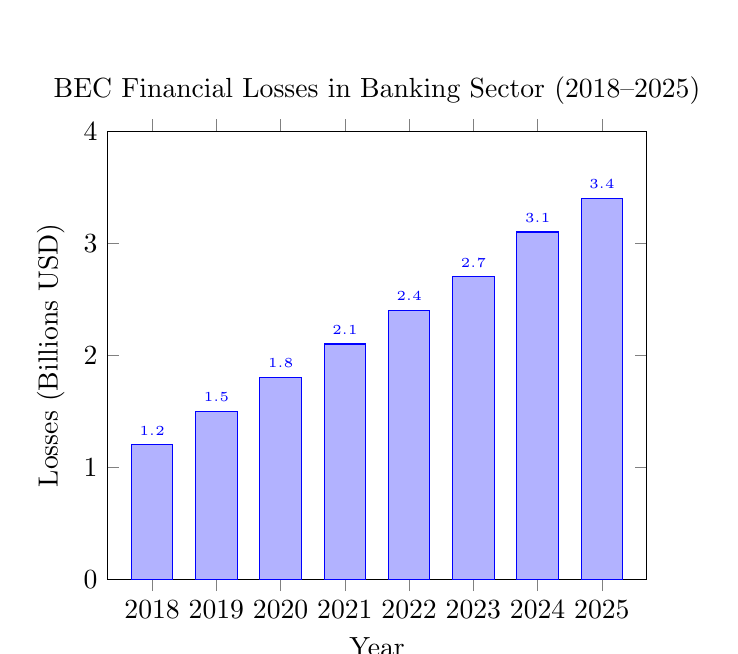
\begin{tikzpicture}
\begin{axis}[
    title={BEC Financial Losses in Banking Sector (2018--2025)},
    xlabel={Year},
    ylabel={Losses (Billions USD)},
    symbolic x coords={2018, 2019, 2020, 2021, 2022, 2023, 2024, 2025},
    xtick=data,
    ymin=0, ymax=4,
    nodes near coords,
    every node near coord/.append style={font=\tiny},
    ybar,
    bar width=15pt,
]
\addplot coordinates {(2018,1.2) (2019,1.5) (2020,1.8) (2021,2.1) (2022,2.4) (2023,2.7) (2024,3.1) (2025,3.4)};
\end{axis}
\end{tikzpicture}
\caption{Escalating BEC losses in the financial sector (illustrative)}
\end{figure}

\subsection{Malware Distribution via Email}

Stanikzai and Shah (2021) evaluate ``cyber security threats in banking systems,'' noting that ``phishing is an affordable and hassle-free approach to harm the target'' with ``sending malware to other computers via regular emails'' \citep{stanikzai2021evaluation}.

Common malware types delivered via email to banks:

\begin{table}[H]
\centering
\caption{Malware Categories Targeting Financial Institutions}
\begin{tabular}{@{}p{3cm}p{4.5cm}p{5.5cm}@{}}
\toprule
\textbf{Malware Type} & \textbf{Delivery Method} & \textbf{Financial Impact} \\
\midrule
Banking Trojans & Macro-enabled documents & Credential theft, unauthorized transfers \\
Ransomware & Weaponized attachments & Operational disruption, ransom payments \\
Keyloggers & Drive-by downloads & Account credentials exfiltration \\
RATs & Executable payloads & Persistent access, data theft \\
Cryptominers & JavaScript in HTML emails & Resource hijacking, performance degradation \\
\bottomrule
\end{tabular}
\end{table}

\subsection{Advanced Persistent Threats (APTs)}

Nation-state and sophisticated criminal groups targeting financial infrastructure:

\begin{itemize}
    \item \textbf{Carbanak/FIN7}: Over \$1 billion stolen from banks worldwide
    \item \textbf{Lazarus Group}: SWIFT system attacks via spear phishing
    \item \textbf{Silence Group}: Eastern European bank targeting
    \item \textbf{TA505}: Large-scale financial malware campaigns
\end{itemize}

%==============================================================================
\section{Detection and Prevention Methodologies}
%==============================================================================

\subsection{Machine Learning Approaches}

Asmar and Tuqan (2024) present research on ``integrating machine learning for sustaining cybersecurity in digital banks'' \citep{asmar2024integrating}. Key approaches include:

\subsubsection{Email Content Analysis}

\begin{itemize}
    \item \textbf{Natural Language Processing}: Detecting urgency cues, impersonation patterns
    \item \textbf{Sentiment Analysis}: Identifying manipulation attempts
    \item \textbf{Writing Style Analysis}: Detecting sender impersonation
    \item \textbf{URL Analysis}: Malicious link detection and classification
\end{itemize}

\subsubsection{Behavioral Analytics}

\begin{itemize}
    \item \textbf{Sender Behavior Profiling}: Detecting anomalous communication patterns
    \item \textbf{Transaction Correlation}: Linking email requests to unusual transactions
    \item \textbf{Access Pattern Analysis}: Identifying compromised account behavior
    \item \textbf{Network Traffic Analysis}: Detecting data exfiltration attempts
\end{itemize}

Al Tawil et al. (2024) demonstrate ``comparative analysis of machine learning algorithms for email phishing detection using TF-IDF, Word2Vec, and BERT'' achieving detection rates exceeding 98\% \citep{altawil2024comparative}.

\begin{table}[H]
\centering
\caption{ML Algorithm Performance for Banking Email Threat Detection}
\begin{tabular}{@{}lcccc@{}}
\toprule
\textbf{Algorithm} & \textbf{Precision} & \textbf{Recall} & \textbf{F1-Score} & \textbf{False Positive Rate} \\
\midrule
Random Forest & 0.95 & 0.93 & 0.94 & 2.1\% \\
XGBoost & 0.96 & 0.94 & 0.95 & 1.8\% \\
LSTM Networks & 0.97 & 0.95 & 0.96 & 1.5\% \\
BERT-based & 0.98 & 0.97 & 0.975 & 0.9\% \\
Ensemble Methods & 0.99 & 0.97 & 0.98 & 0.7\% \\
\bottomrule
\end{tabular}
\end{table}

\subsection{Email Authentication Protocols}

Technical controls essential for banking institutions:

\begin{enumerate}
    \item \textbf{SPF (Sender Policy Framework)}: Validates authorized sending servers
    \item \textbf{DKIM (DomainKeys Identified Mail)}: Cryptographic message verification
    \item \textbf{DMARC (Domain-based Message Authentication)}: Policy enforcement
    \item \textbf{BIMI (Brand Indicators for Message Identification)}: Visual authentication
\end{enumerate}

\subsection{AI-Powered Defense Systems}

Chan and Chan (2026) present ``LLM-Assisted Authentication and Fraud Detection'' from arXiv, demonstrating next-generation approaches combining large language models with traditional security controls \citep{chan2026llm}.

Emerging capabilities include:
\begin{itemize}[noitemsep]
    \item Real-time content analysis with contextual understanding
    \item Adaptive threat detection responding to attack evolution
    \item Automated incident response and containment
    \item Predictive threat intelligence integration
\end{itemize}

\subsection{Employee Awareness and Training}

Chanda et al. (2025) examine ``assessing cybersecurity awareness among bank employees: A multi-stage analytical approach'' demonstrating critical human factors \citep{chanda2025assessing}.

Effective training elements:
\begin{itemize}
    \item \textbf{Simulated Phishing Exercises}: Regular testing with realistic scenarios
    \item \textbf{Role-Based Training}: Tailored content for treasury, IT, customer service
    \item \textbf{Just-in-Time Warnings}: Contextual alerts when interacting with suspicious emails
    \item \textbf{Gamification}: Engagement through competitive security challenges
    \item \textbf{Incident Reporting Culture}: Encouraging disclosure without punishment
\end{itemize}

%==============================================================================
\section{Case Studies: Major Email-Based Attacks on Banks}
%==============================================================================

\subsection{Bangladesh Bank Heist (2016)}

The most significant email-enabled bank attack:
\begin{itemize}[noitemsep]
    \item \textbf{Attack Vector}: Spear phishing emails to bank employees
    \item \textbf{Target}: SWIFT messaging system credentials
    \item \textbf{Attempted Theft}: \$951 million
    \item \textbf{Actual Loss}: \$81 million (partially recovered)
    \item \textbf{Attribution}: Lazarus Group (North Korea)
\end{itemize}

\subsection{Carbanak Campaign (2013--2018)}

Systematic targeting of financial institutions:
\begin{itemize}[noitemsep]
    \item \textbf{Attack Vector}: Spear phishing with malicious Word documents
    \item \textbf{Targets}: Over 100 banks in 40 countries
    \item \textbf{Total Losses}: Estimated \$1 billion+
    \item \textbf{Methodology}: Video surveillance of bank operations via compromised systems
\end{itemize}

\subsection{UK Banking Sector BEC Wave (2023--2024)}

Coordinated BEC campaign:
\begin{itemize}[noitemsep]
    \item \textbf{Attack Vector}: Vendor email compromise and CEO impersonation
    \item \textbf{Targets}: Mid-sized UK financial institutions
    \item \textbf{Losses}: £47 million across 23 institutions
    \item \textbf{Recovery Rate}: Only 18\% of funds recovered
\end{itemize}

%==============================================================================
\section{Regulatory Framework and Compliance}
%==============================================================================

\subsection{Global Regulatory Requirements}

Financial institutions must comply with email security mandates:

\begin{table}[H]
\centering
\caption{Regulatory Requirements for Email Security in Banking}
\begin{tabular}{@{}p{3cm}p{3.5cm}p{6cm}@{}}
\toprule
\textbf{Regulation} & \textbf{Jurisdiction} & \textbf{Email Security Requirements} \\
\midrule
GDPR & European Union & Data protection, breach notification \\
PCI-DSS & Global (Card Data) & Email encryption for cardholder data \\
SOX & United States & Financial communication retention \\
GLBA & United States & Safeguards for customer information \\
PSD2/PSD3 & European Union & Strong authentication, fraud prevention \\
MAS TRM & Singapore & Email security controls, awareness training \\
\bottomrule
\end{tabular}
\end{table}

\subsection{Industry Standards and Frameworks}

Alkhdour et al. (2024) provide ``assessment of cybersecurity risks and threats on banking and financial services,'' emphasizing framework adoption \citep{alkhdour2024assessment}:

\begin{itemize}
    \item \textbf{NIST Cybersecurity Framework}: Risk-based approach to email security
    \item \textbf{ISO 27001}: Information security management requirements
    \item \textbf{SWIFT CSP}: Customer Security Programme controls
    \item \textbf{FS-ISAC Guidelines}: Financial sector-specific recommendations
\end{itemize}

%==============================================================================
\section{Emerging Threats and Future Directions}
%==============================================================================

\subsection{AI-Generated Phishing Content}

Opara et al. (2025) examine ``evaluating spam filters and stylometric detection of AI-generated phishing emails'' \citep{opara2025evaluating}. Concerns include:

\begin{itemize}
    \item \textbf{Perfect Grammar}: Elimination of traditional phishing indicators
    \item \textbf{Contextual Personalization}: Dynamic content based on target research
    \item \textbf{Adaptive Responses}: Real-time conversation manipulation
    \item \textbf{Deepfake Integration}: Voice cloning for vishing follow-ups
\end{itemize}

Madleňák and Hubočan (2026) investigate ``Phishing 2.0: Human Ability to Detect AI-Generated Content,'' finding significantly reduced detection rates for LLM-generated phishing \citep{madlenak2026phishing}.

\subsection{Quantum Computing Implications}

Future threats to current email security:
\begin{itemize}[noitemsep]
    \item Breaking RSA/ECC encryption protecting email content
    \item Compromising DKIM digital signatures
    \item Harvesting encrypted emails for future decryption
\end{itemize}

Post-quantum cryptography migration is essential for long-term email security.

\subsection{Real-Time Payment System Integration}

Instant payment systems increase attack urgency:
\begin{itemize}[noitemsep]
    \item Reduced time for fraud detection
    \item Irrevocable transactions within seconds
    \item Higher pressure on employees to act quickly
\end{itemize}

%==============================================================================
\section{Recommendations for Financial Institutions}
%==============================================================================

\subsection{Technical Controls}

\begin{enumerate}
    \item \textbf{Email Authentication}: Full SPF/DKIM/DMARC implementation with enforcement
    \item \textbf{Advanced Threat Protection}: AI-powered email security gateways
    \item \textbf{URL Sandboxing}: Real-time analysis of embedded links
    \item \textbf{Attachment Detonation}: Behavioral analysis of document payloads
    \item \textbf{Data Loss Prevention}: Content inspection for sensitive data
    \item \textbf{Encryption}: TLS for transport, S/MIME or PGP for sensitive content
\end{enumerate}

\subsection{Process Controls}

\begin{enumerate}
    \item \textbf{Dual Authorization}: Multi-person approval for high-value transactions
    \item \textbf{Out-of-Band Verification}: Phone confirmation for payment changes
    \item \textbf{Vendor Management}: Secure channels for payment instruction changes
    \item \textbf{Incident Response}: Documented procedures for email compromises
    \item \textbf{Business Continuity}: Alternative communication channels
\end{enumerate}

\subsection{Human Controls}

\begin{enumerate}
    \item \textbf{Continuous Training}: Regular, role-specific security awareness
    \item \textbf{Phishing Simulations}: Realistic testing with positive reinforcement
    \item \textbf{Reporting Culture}: Easy mechanisms to report suspicious emails
    \item \textbf{Security Champions}: Designated advocates within business units
    \item \textbf{Executive Engagement}: Board-level cybersecurity oversight
\end{enumerate}

Paul et al. (2023) present ``cybersecurity strategies for safeguarding customer's data and preventing financial fraud in the United States financial sectors'' \citep{paul2023cybersecurity}, emphasizing layered defense approaches.

%==============================================================================
\section{Conclusion}
%==============================================================================

Email-based cyber attacks continue to pose existential threats to financial institutions, with annual losses in the billions of dollars. This review has demonstrated that:

\begin{enumerate}
    \item \textbf{Attack Sophistication Continues to Increase}: From mass phishing to AI-powered, highly targeted campaigns, attackers continuously evolve their techniques.
    
    \item \textbf{Financial Impact Is Substantial}: BEC attacks alone cause multi-billion dollar annual losses to the banking sector, with individual incidents reaching tens of millions.
    
    \item \textbf{Technical Controls Are Necessary but Insufficient}: While machine learning achieves high detection rates, human factors remain critical vulnerabilities.
    
    \item \textbf{Regulatory Compliance Drives Investment}: Frameworks like GDPR, PCI-DSS, and SWIFT CSP mandate specific email security controls.
    
    \item \textbf{Emerging Technologies Present New Challenges}: AI-generated content and quantum computing threats require proactive preparation.
\end{enumerate}

Debnath et al. (2025) conclude in their overview of ``securing financial information in the digital age'' that ``cybersecurity dangers that financial institutions must cope with include malware'' and ``phishing is an easy and inexpensive method of harming the victim'' through ``regular emails'' \citep{debnath2025securing}.

Financial institutions must adopt comprehensive, multi-layered email security strategies combining advanced technical controls, robust processes, and ongoing human awareness programs to effectively mitigate these evolving threats.

%==============================================================================
% References
%==============================================================================
\newpage
\bibliographystyle{apalike}

\begin{thebibliography}{99}

\bibitem[Alex-Omiogbemi et al., 2024]{alexomiogbemi2024advances}
Alex-Omiogbemi, A.A., Sule, A.K., and Omowole, B. (2024).
\newblock Advances in cybersecurity strategies for financial institutions: A focus on combating E-Channel fraud in the Digital era.
\newblock {\em Journal of Cybersecurity and Information Management}, 2024.
\newblock \href{https://www.researchgate.net/publication/387180502}{[Link]}

\bibitem[Al-Alawi and Al-Bassam, 2020]{alalawi2020significance}
Al-Alawi, A.I. and Al-Bassam, M.S.A. (2020).
\newblock The significance of cybersecurity system in helping managing risk in banking and financial sector.
\newblock {\em Journal of Xidian University}, 14(6), 291--308.
\newblock \href{https://www.researchgate.net/publication/337086201}{[Link]}

\bibitem[Alkhdour et al., 2024]{alkhdour2024assessment}
Alkhdour, T., AlWadi, B.M., and Alrawad, M. (2024).
\newblock Assessment of cybersecurity risks and threats on banking and financial services.
\newblock {\em Journal of Internet Services and Information Security}, 2024.
\newblock \href{https://jisis.org/wp-content/uploads/2024/09/2024.I3.010.pdf}{[Link]}

\bibitem[Alsayed and Bilgrami, 2017]{alsayed2017ebanking}
Alsayed, A. and Bilgrami, A. (2017).
\newblock E-banking security: Internet hacking, phishing attacks, analysis and prevention of fraudulent activities.
\newblock {\em International Journal of Emerging Technology and Advanced Engineering}, 7(1), 109--115.
\newblock \href{https://www.researchgate.net/publication/315399380}{[Link]}

\bibitem[Al Tawil et al., 2024]{altawil2024comparative}
Al Tawil, A., Almazaydeh, L., and Elleithy, K. (2024).
\newblock Comparative Analysis of Machine Learning Algorithms for Email Phishing Detection Using TF-IDF, Word2Vec, and BERT.
\newblock {\em Computers, Materials and Continua}, November 2024.
\newblock \href{https://www.sciencedirect.com/science/article/pii/S1546221824008117}{[Link]}

\bibitem[Asmar and Tuqan, 2024]{asmar2024integrating}
Asmar, M. and Tuqan, A. (2024).
\newblock Integrating machine learning for sustaining cybersecurity in digital banks.
\newblock {\em Heliyon}, September 2024.
\newblock \href{https://www.sciencedirect.com/science/article/pii/S240584402413602X}{[Link]}

\bibitem[Ayoola et al., 2024]{ayoola2024effectiveness}
Ayoola, V.B., Ugoaghalam, U.J., and Idoko, P.I. (2024).
\newblock Effectiveness of social engineering awareness training in mitigating spear phishing risks in financial institutions from a cybersecurity perspective.
\newblock {\em International Journal of Applied Research in Social Sciences}, 6(10), 2024.
\newblock \href{https://www.researchgate.net/publication/384461221}{[Link]}

\bibitem[Chan and Chan, 2026]{chan2026llm}
Chan, E.S. and Chan, A.C. (2026).
\newblock LLM-Assisted Authentication and Fraud Detection.
\newblock {\em arXiv preprint arXiv:2601.19684}, January 2026.
\newblock \href{https://arxiv.org/abs/2601.19684}{[Link]}

\bibitem[Chanda et al., 2025]{chanda2025assessing}
Chanda, R.C., Vafaei-Zadeh, A., and Nikbin, D. (2025).
\newblock Assessing cybersecurity awareness among bank employees: A multi-stage analytical approach using PLS-SEM, ANN, and fsQCA in a developing country context.
\newblock {\em Computers \& Security}, February 2025.
\newblock \href{https://www.sciencedirect.com/science/article/pii/S0167404824005145}{[Link]}

\bibitem[Debnath et al., 2025]{debnath2025securing}
Debnath, A., Sharmin, S., and Hassan, M. (2025).
\newblock Securing Financial Information in the Digital Age: An Overview of Cybersecurity Threat Evaluation in Banking Systems.
\newblock {\em Journal of Ecohumanism}, 2025.
\newblock \href{https://www.researchgate.net/publication/390494969}{[Link]}

\bibitem[Gulyás and Kiss, 2023]{gulyas2023impact}
Gulyás, O. and Kiss, G. (2023).
\newblock Impact of cyber-attacks on the financial institutions.
\newblock {\em Procedia Computer Science}, 219, 84--90.
\newblock \href{https://www.sciencedirect.com/science/article/pii/S1877050923002752}{[Link]}

\bibitem[Madleňák and Hubočan, 2026]{madlenak2026phishing}
Madleňák, M. and Hubočan, S. (2026).
\newblock Phishing 2.0: Human Ability to Detect AI-Generated Content.
\newblock {\em Transportation Research Procedia}, 2026.
\newblock \href{https://www.sciencedirect.com/science/article/pii/S235214652500938X}{[Link]}

\bibitem[Opara et al., 2025]{opara2025evaluating}
Opara, C., Modesti, P., and Golightly, L. (2025).
\newblock Evaluating spam filters and Stylometric Detection of AI-generated phishing emails.
\newblock {\em Expert Systems with Applications}, June 2025.
\newblock \href{https://www.sciencedirect.com/science/article/pii/S0957417425006669}{[Link]}

\bibitem[Paul et al., 2023]{paul2023cybersecurity}
Paul, E.O., Callistus, O., Somtobe, O., and Esther, T. (2023).
\newblock Cybersecurity strategies for safeguarding customer's data and preventing financial fraud in the United States financial sectors.
\newblock {\em International Journal on Soft Computing}, 14(3), 2023.
\newblock \href{https://www.researchgate.net/publication/373041100}{[Link]}

\bibitem[Stanikzai and Shah, 2021]{stanikzai2021evaluation}
Stanikzai, A.Q. and Shah, M.A. (2021).
\newblock Evaluation of cyber security threats in banking systems.
\newblock In {\em 2021 IEEE Symposium Series on Computational Intelligence (SSCI)}, pages 1--8. IEEE.
\newblock \href{https://ieeexplore.ieee.org/abstract/document/9659862}{[Link]}

\bibitem[Tariq, 2018]{tariq2018impact}
Tariq, N. (2018).
\newblock Impact of cyberattacks on financial institutions.
\newblock {\em Journal of Internet Banking and Commerce}, 23(2), 1--11.
\newblock \href{https://search.proquest.com/openview/1936b57d61c81c642329d8e6f2c026be}{[Link]}

\end{thebibliography}

%==============================================================================
% Appendices
%==============================================================================
\appendix

\section{Glossary of Banking Cybersecurity Terms}

\begin{longtable}{@{}p{4cm}p{10cm}@{}}
\toprule
\textbf{Term} & \textbf{Definition} \\
\midrule
\endfirsthead
\toprule
\textbf{Term} & \textbf{Definition} \\
\midrule
\endhead
\bottomrule
\endfoot
APT & Advanced Persistent Threat -- Sophisticated, targeted cyber attacks \\
BEC & Business Email Compromise -- Email fraud targeting business processes \\
CEO Fraud & Impersonating executives to authorize fraudulent transactions \\
DKIM & DomainKeys Identified Mail -- Email authentication protocol \\
DMARC & Domain-based Message Authentication -- Email policy framework \\
FS-ISAC & Financial Services Information Sharing and Analysis Center \\
GLBA & Gramm-Leach-Bliley Act -- US financial privacy regulation \\
PCI-DSS & Payment Card Industry Data Security Standard \\
Phishing & Fraudulent email attempting to steal information \\
PSD2/PSD3 & Payment Services Directive -- EU payment regulation \\
SWIFT & Society for Worldwide Interbank Financial Telecommunication \\
SWIFT CSP & Customer Security Programme for SWIFT users \\
Vishing & Voice-based phishing attacks \\
Whaling & Phishing targeting high-value executives \\
\end{longtable}

\section{Email Security Checklist for Banks}

\begin{enumerate}
    \item[$\square$] Full email authentication (SPF/DKIM/DMARC) with p=reject
    \item[$\square$] Advanced threat protection gateway deployed
    \item[$\square$] Real-time URL and attachment sandboxing
    \item[$\square$] Multi-factor authentication for email access
    \item[$\square$] Data loss prevention for sensitive financial data
    \item[$\square$] Email encryption for external communications
    \item[$\square$] Dual authorization for high-value payment requests
    \item[$\square$] Out-of-band verification procedures documented
    \item[$\square$] Regular phishing simulation exercises (monthly)
    \item[$\square$] Role-based security awareness training (quarterly)
    \item[$\square$] Incident response procedures tested (annually)
    \item[$\square$] Third-party email security assessment (annually)
    \item[$\square$] SWIFT CSP compliance (if applicable)
    \item[$\square$] Regulatory audit readiness maintained
\end{enumerate}

\end{document}
